\documentclass{article}
\usepackage{fancyhdr}
\usepackage{graphicx}
\usepackage{amsmath}
\usepackage{xcolor}
\usepackage{caption}
\usepackage{amssymb}

\usepackage[margin=1in]{geometry}
\usepackage{cancel} 

\pagestyle{fancy}
\graphicspath{ {./img/} }

\begin{document}
	\begin{titlepage}
		\begin{center}
			\vspace{1cm}
			{\LARGE\textbf{Amplifier Project}}
			
			\vspace{1.5cm}
			\textbf{\large Ghassan Arnouk}\\
			
			\vspace{1cm}
			\large ELEC 3509B\\
			\large Summer 2020\\
			\large Lab 2 Report\\
			
			
			\vspace{2cm}
			\textbf{Instructor:} Qi-Jun Zhang\\
			
			
			\vspace{1cm}
			\textbf{Lab Period:} B1\\
			
			\vspace{0.1cm}
			\textbf{Day 1 Preformed:} 2020/07/16
			
			\vspace{0.1cm}
			\textbf{Day 2 Preformed:} 2020/07/22

			\vspace{0.1cm}
			\textbf{Day 3 Preformed:} 2020/07/23
			
			\vspace{1cm}
			\textbf{Date Submitted:} 2020/07/30\\			
		\end{center}
	\end{titlepage}
	
	\lhead{Ghassan Arnouk (B1)}
	\rhead{Amplifier Project}
	\pagebreak
	
	\tableofcontents
	\pagebreak
	
	\listoftables
	\pagebreak
	
	\listoffigures
	\pagebreak
	
	\section{Introduction}
	\subsection{Purpose}
	The purpose of this lab is to investigate the use of BJTs as amplifier circuit elements [1].
	First, the three basic configurations (CE, CC, and CB) are observed [1].
	Then, by proper combinations and permutations, 2-transistor amplifier configurations can be studied for improved gain-bandwidth performance [1].
	Finally, a specific configuration was required to be designed to meet or exceed a prescribed set of specifications [1].
	
	\subsection{Experiment Overview}
	In day 1, three different signle amplifier configurations and three different two-transsitor configurations were constrcuted and analyzed.
	Data were measured and the charactersitics of the amplifiers were verified.
	Then, useful parameters were calculated using the obtained measurements.\\\\
	In day 2, a cascode amplifier design is constructed and tested.
	Data were measured to verify that the measured parameters values of the cascode amplifier matched with the assumptions and the theoretical calculations when analyzing the amplifier.\\\\
	In day 3, more test measurments were done to verify the functionality of the designed cascode amplifier as well as to confirm that the design meet or exceed a prescribed set of specifications.

	\section{Background}
	The semiconductor device introduced in this course is the bipolar junction transistor.
	The three basic configurations of the BJT amplifier are the common-collector mode, common-base mode, and common-emitter mode.
	These configurations are used for voltage or current amplification.
	However, the various configurations can be combined to create two-transistor amplifiers which overcome the drawbacks of the single transistor amplifiers and provide more desireable characteristics analog designers seek.
	
	\pagebreak
	\section{Cascode Amplifier Design Project}
	\subsection{Prelab}
	$$Z = 5  + 5 + 0 = 10$$
	\subsection*{Design Requirements:}
	\begin{enumerate}
		\item Mangnitude of voltage gain: $$|A_v| = 12\sqrt{10 + 35} = 12\sqrt{45} = 80.50 \hspace{1mm} v/v \pm 10\% = (80.50 \pm 8.05) \hspace{1mm} v/v$$
		\item Load resistance: $$R_L = 6(10 + 40)^{2} = 6(50)^{2} = 15 \hspace{1mm} k\Omega$$
		\item The high frequency cutoff $f_H$ is to be maximized. \textbf{It must exceed 1 MHz}.
		\item The output voltage: $V_{out}$ = approximately 2 V peak-peak without appreciable distortion.
		\begin{itemize}
			\item To ensure this, the AC base-emitter voltage must be kept under 10 mV peak-peak for such an output.
		\end{itemize}
		\item No DC current may flow in $R_L$ and no DC current may flow into or out of the signal generator.
		\item The low frequency \textbf{$f_L$ must be less than 200 Hz}.
		\item The magnitudes of the input and output impedances at 1 kHz are to be determined by calculation and then measured.
		\item Total circuit power \textbf{is not to exceed 50 m}W.
		\item The transistors are all to be 2N3904.
		\item Collector currents in the transistors are to be $1.0 \hspace{1mm} mA \pm 10\% = (1.0 \pm 0.1) \hspace{1mm} mA$.
		\item Power-supply voltages are to be \textbf{+15 volts}.
		\item No adjustable components, e.g. trim-pots, will be allowed.
		\item Additional design requirements:		
		$$\beta = 147.06$$
		$$\alpha = 0.99 \approx 1$$
		$$C_{\mu} = 4 \hspace{1mm} pf$$
		$$C_{\pi} \approx 50 \hspace{1mm} pf$$
		$$g_m = 40 \hspace{1mm} milli \hspace{1mm} mhos$$
		$$r_{\pi} = 3.313 \hspace{1mm} k\Omega$$
		$$r_e = \frac{\alpha}{g_m} = \frac{0.99}{40 \hspace{1mm} milli \hspace{1mm} mhos} = 24.75 \hspace{1mm} \Omega$$			
	\end{enumerate}		
	\pagebreak		
	Figure \ref{f1} below shows an example schematic of a cascode amplifier circuit.
	\begin{figure}[!ht]
		\centering
		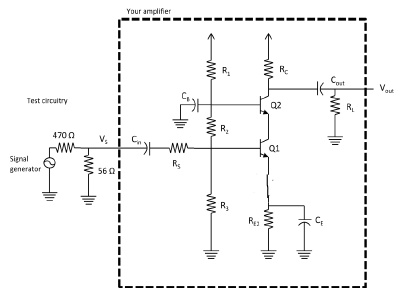
\includegraphics[width=\linewidth]{cascode_schematic.png}
		\captionof{figure}{Schematic of Cascode Amplifier Circuit [1]}\label{f1}
	\end{figure}
	\pagebreak
	\subsection*{DC Analysis:}
	Assuming $V_{E}$ is 20\% of $V_{CC}$, we get the following:
	\begin{align*}
		V_{E} &= 0.2 * V_{CC}\\
				&= 0.2 * 15 \hspace{1mm} V\\
				&= 3 \hspace{1mm} V
	\end{align*}
	\noindent Assuming $V_{CE_{1}} = 2 \hspace{1mm} V$, we get the following:
	\begin{align*}
		V_{C_1} &= V_{E_1} + V_{CE_1}\\
		&= 3 \hspace{1mm} V + 2 \hspace{1mm} V\\
		&= 5 \hspace{1mm} V
	\end{align*}
	\begin{align*}
		V_{C_2} &= \frac{V_{CC} + V_{C_1}}{2}\\
		&= \frac{15 \hspace{1mm} V + \hspace{1mm} 5 \hspace{1mm} V}{2}\\
		&= 10 \hspace{1mm} V
	\end{align*}
	Based on these assumptions, we can calculate all of the followings:
	\begin{align*}
		R_{E_2} &= \frac{V_{E}}{I_{E}}\\
		&= \frac{3 \hspace{1mm} V}{1 \hspace{1mm} mA}\\ 
		&= 3 \hspace{1mm} k\Omega
	\end{align*}
	\begin{align*}
		R_C &= \frac{V_{CC} - V_{C_2}}{I_{C_2}}\\ 
		&= \frac{15 \hspace{1mm} V - \hspace{1mm} 10 \hspace{1mm} V}{1 \hspace{1mm} mA}\\ 
		&= 5 \hspace{1mm} k\Omega
	\end{align*}
	\begin{align*}
		V_{B_1} &= V_{E_1} + 0.7 \hspace{1mm} V\\
		&= 3 \hspace{1mm} V + 0.7\\ 
		&= 3.7 \hspace{1mm} V
	\end{align*}
	\begin{align*}
		V_{B_2} &= V_{C_1} + 0.7 \hspace{1mm} V\\ 
		&= 5 \hspace{1mm} V + 0.7\\ 
		&= 5.7 \hspace{1mm} V
	\end{align*}
	Given the values of $I_C$ and $\beta$ from Lab 1 report, we get the following:
	\begin{align*}
		I_{B_1} &= I_{B_2} = \frac{I_C}{\beta}\\
		&= \frac{1 \hspace{1mm} mA}{147.06}\\
		&= 6.8 \hspace{1mm}\mu A
	\end{align*}
	Assuming $I_{BB}$ is ten times the sum of the base currents of both transistors, we get the following:
	\begin{align*}
		I_{BB} &= 10 * (I_{B_1} + I_{B_2})\\ 
		&= 10 * (6.8 \hspace{1mm}\mu A + 6.8 \hspace{1mm}\mu A)\\ 
		&= 10 * (13.6 \hspace{1mm}\mu A)\\ 
		&= 136 \hspace{1mm}\mu A
	\end{align*}
	Based on the previous calculations, $R_1$, $R_2$, $R_3$, can be calculated as follows:
	\begin{align*}
		R_1 &= \frac{V_{CC} - V_{B_2}}{I_{BB}}\\ 
		&= \frac{15 \hspace{1mm} V - \hspace{1mm} 5.7 \hspace{1mm} V}{136 \hspace{1mm}\mu A}\\ 
		&\approx 68.40 \hspace{1mm} k\Omega
	\end{align*}
	\begin{align*}
		R_2 &= \frac{V_{B_2} - \hspace{1mm} V_{B_1}}{I_{BB} - \hspace{1mm} I_{B_2}}\\ 
		&= \frac{5.7 \hspace{1mm} V - \hspace{1mm} 3.7 \hspace{1mm} V}{136 \hspace{1mm}\mu A - \hspace{1mm} 6.8 \hspace{1mm}\mu A}\\ 
		&\approx 15.5 \hspace{1mm} k\Omega
	\end{align*}
	\begin{align*}
		R_3 &= \frac{V_{B_1}}{I_{BB} - \hspace{1mm} I_{B_1} - \hspace{1mm} I_{B_2}}\\
		&= \frac{3.7 \hspace{1mm} V}{136 \hspace{1mm}\mu A - \hspace{1mm} 6.8 \hspace{1mm}\mu A - \hspace{1mm} 6.8 \hspace{1mm}\mu A}\\ 
		&\approx 30.23 \hspace{1mm} k\Omega
	\end{align*}
	
	\pagebreak
	Figure \ref{f2} below shows an example schematic of the designed cascode amplifier circuit.
	\begin{figure}[!ht]
		\centering
		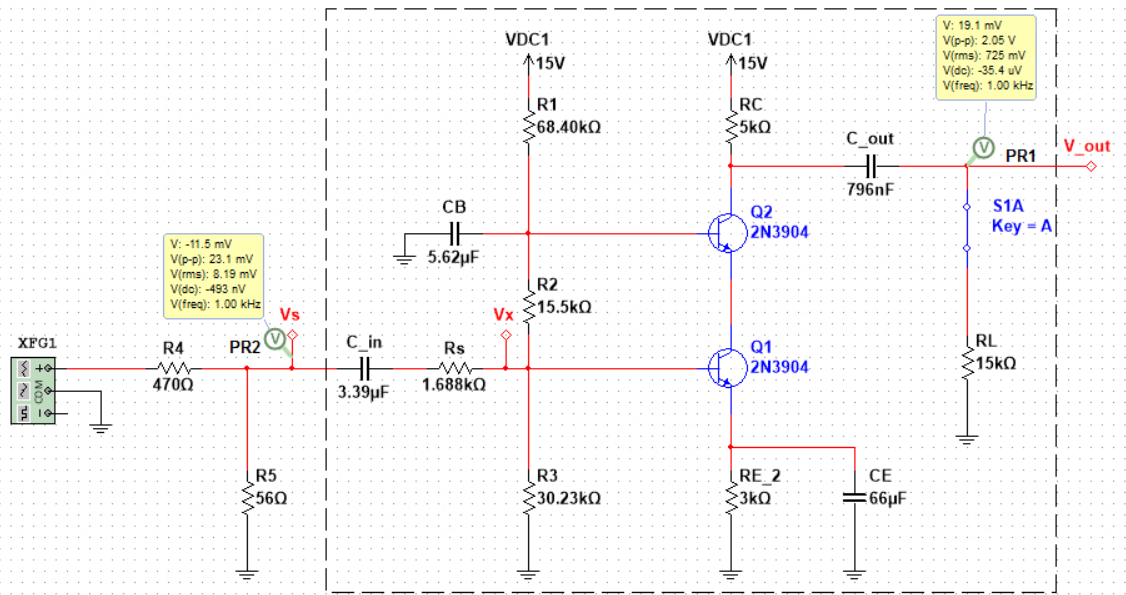
\includegraphics[width=\linewidth]{cascode_schematic_values.png}
		\captionof{figure}{Schematic of The Designed Cascode Amplifier Circuit [1]}
		\label{f2}
	\end{figure}
	\pagebreak
	\subsection*{AC Analysis:}
	Figure \ref{f:1} below shows the small signal model of the cascode amplifier project.
	\begin{figure}[!ht]
		\centering
		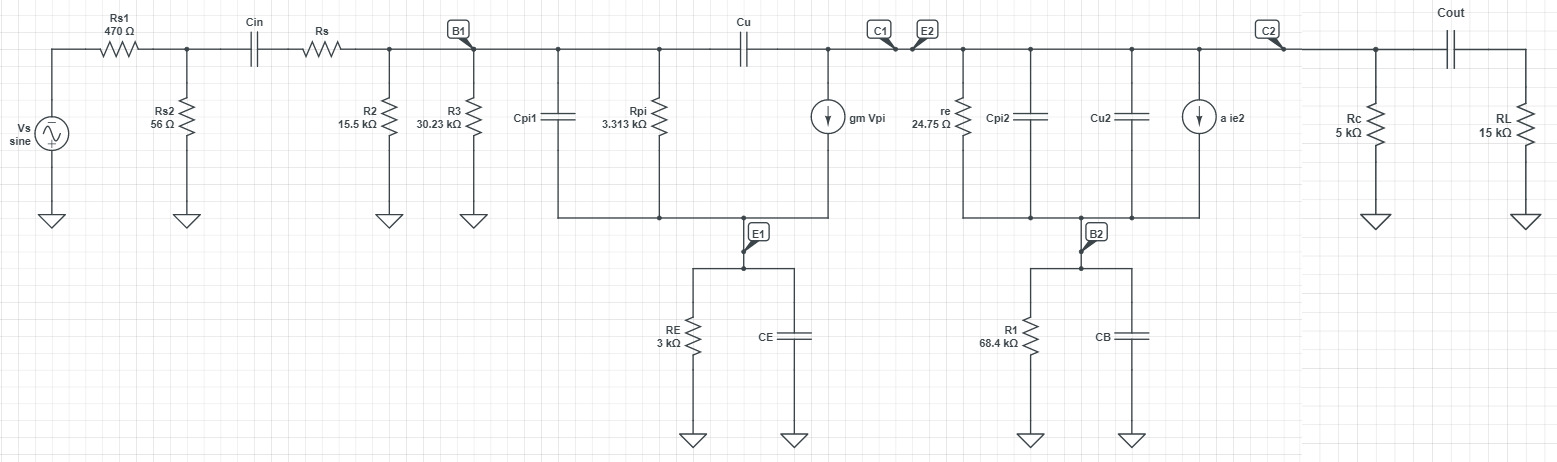
\includegraphics[width=\linewidth]{ssm.png}
		\captionof{figure}{The Small Signal Model of The Cascode Amplifier Project}
		\label{f:1}
	\end{figure}
	
	\noindent\textbf{Step 1:} $A_v$\\ $$|A_v| = 12\sqrt{10 + 35} = 12\sqrt{45} = 80.50 \hspace{1mm} v/v \pm 10\% = (80.50 \pm 8.05) \hspace{1mm} v/v$$
	\noindent The voltage gain is derived as follows:
	\begin{align*}
		A_v &= \frac{-\alpha i_{E_2} (R_C // R_L)} {V_{\pi}} * \frac{\frac{R_2 // R_S // r_{\pi}}{R_{S_1} + \hspace{1mm}R_S + \hspace{1mm} [R_2 // R_3 // r_{\pi}]} * V_S}{V_S}\\
		&= \frac{\alpha g_m \cancel{V_{\pi}} (R_C // R_L)} {\cancel{V_{\pi}}} * \frac{\frac{R_2 // R_S // r_{\pi}}{R_{S_1} + \hspace{1mm}R_S + \hspace{1mm}[R_2 // R_3 // r_{\pi}]} * \cancel{V_S}}{\cancel{V_S}}\\
		A_v &= \alpha g_m (R_C // R_L) * \frac{R_2 // R_S // r_{\pi}}{R_{S_1} + \hspace{1mm}R_S + \hspace{1mm}[R_2 // R_3 // r_{\pi}]}
	\end{align*}
	\noindent By rearranging the previous equation for $R_S$, we get the following:
	\begin{align*}
		R_S &= \frac{[\alpha g_m (R_C // R_L)] [R_2 // R_3 // r_{\pi}]}{A_v} - \hspace{1mm} R_{S_1} - \hspace{1mm} (R_2 // R_3 // r_{\pi})\\
		&= \frac{[(1)(40 \hspace{1mm} milli \hspace{1mm} mhos) (5 \hspace{1mm} k\Omega // 15 \hspace{1mm} k\Omega)] [15.5 \hspace{1mm} k\Omega // 30.23 \hspace{1mm} k\Omega // 3.313 \hspace{1mm} k\Omega]}{80.50} - \hspace{1mm} 470 \hspace{1mm} \Omega - \hspace{1mm} (15.5 \hspace{1mm} k\Omega // 30.23 \hspace{1mm} k\Omega // 3.313 \hspace{1mm} k\Omega)\\
		&= 1.688 \hspace{1mm} k\Omega
	\end{align*}
	\textbf{Setp 2:} $R_{in}$
	\begin{align*}
		R_{in} &= R_S + (R_2 // R_3 // r_{\pi})\\
		&= 1.688 \hspace{1mm} k\Omega + (15.5 \hspace{1mm} k\Omega // 30.23 \hspace{1mm} k\Omega // 3.313 \hspace{1mm} k\Omega)\\
		&= 4.188 \hspace{1mm} k\Omega
	\end{align*}
	\textbf{Setp 3:} $R_{out}$
	\begin{align*}
		R_{out} = R_C = 5 \hspace{1mm} k\Omega
	\end{align*}
	
	\noindent Assuming a low frequency, $f_L$, of \textbf{100 Hz}, and taking the design considerations below into account:
	\begin{align*}
		&\frac{1}{R_{C_E} C_E} \rightarrow 70\% \hspace{1mm} of \hspace{1mm} 2\pi f_L\\
		&\frac{1}{R_{C_B} C_B} = \frac{1}{R_{C_{in}} C_{in}} = \frac{1}{R_{C_{out} C_{out}}} \rightarrow 10\% \hspace{1mm} of \hspace{1mm} 2\pi f_L
	\end{align*}
	
	\pagebreak
	\noindent Then, the capaciotrs can be calculated as follows:\\
	\begin{align*}
		\frac{1}{R_{C_{in}} C_{in}} = 0.1 * 2\pi f_L
	\end{align*}
	\begin{align*}
		R_{C_{in}} &= [R_{S_1} // R_{S_2}] + R_s + [R_2 // R_3 // r_{\pi}]\\
		&= [470 \hspace{1mm} \Omega // 56 \hspace{1mm} \Omega] + 1.688 \hspace{1mm} k\Omega + [15.5 \hspace{1mm} k\Omega // 30.23 \hspace{1mm} k\Omega // 3.313 \hspace{1mm} k\Omega]\\
		&= 4.688 \hspace{1mm} k\Omega
	\end{align*}
	\begin{align*}
		C_{in} &= \frac{1}{0.1 * (2\pi * 100 \hspace{1mm} Hz) * (4.688 \hspace{1mm} k\Omega)}\\
		&\approx 3.39 \hspace{1mm} \mu F\\ 
	\end{align*}
	
	\begin{align*}
		\frac{1}{R_{C_E} C_E} = 0.7 * 2\pi f_L
	\end{align*}
	\begin{align*}
		R_{C_E} &= R_E // \left[\frac{r_{\pi} + [[({R_{S_1}} // R_{S_2}) + R_S] // R_2 // R_3]}{1 + \beta}\right]\\
		&= 3 \hspace{1mm} k\Omega // \left[\frac{3.313 \hspace{1mm} k\Omega + [[(470 \hspace{1mm} \Omega // 56 \hspace{1mm} \Omega) + 1.688 \hspace{1mm} k\Omega] // 15.5 \hspace{1mm} k\Omega // 30.23 \hspace{1mm} k\Omega]}{1 + 147.06} \right]\\		
		&= 34.21 \hspace{1mm} \Omega
	\end{align*}
	\begin{align*}
		C_E &= \frac{1}{0.7 * (2\pi * 100 \hspace{1mm} Hz) * (34.21 \hspace{1mm} \Omega)}\\
		&\approx 66 \hspace{1mm} \mu F\\
	\end{align*}

	\begin{align*}
		\frac{1}{R_{C_B} C_B} = 0.1 * 2\pi f_L
	\end{align*}
	\begin{align*}
		R_{C_B} &= R_1 // R_2 // [r_e * (1 + \beta)]\\
		&= 68.40 \hspace{1mm} k\Omega // 15.5 \hspace{1mm} k\Omega // [24.75 \hspace{1mm} \Omega * (1 + 147.06)]\\
		&= 2.83 \hspace{1mm} k\Omega
	\end{align*}
	\begin{align*}
		C_B &= \frac{1}{0.1 * (2\pi * 100 \hspace{1mm} Hz) * (2.83 \hspace{1mm} k\Omega)}\\
		&\approx 5.62 \hspace{1mm} \mu F\\
	\end{align*}
	\pagebreak
	\begin{align*}
		\frac{1}{R_{C_{out}} C_{out}} = 0.1 * 2\pi f_L
	\end{align*}
	\begin{align*}
		R_{C_{out}} &= R_C + R_L\\
		&= 5 \hspace{1mm} k\Omega + 15 \hspace{1mm} k\Omega\\
		&= 20 \hspace{1mm} k\Omega
	\end{align*}
	\begin{align*}
		C_B &= \frac{1}{0.1 * (2\pi * 100 \hspace{1mm} Hz) * (20 \hspace{1mm} k\Omega)}\\
		&\approx 796 \hspace{1mm} nF\\
	\end{align*}
	
	\noindent\textbf{Step 4:} Low Poles\\
	\begin{align*}
		\omega_{L_1} &= \frac{1}{2\pi R_{C_{in}} C_{in}}\\
		&= \frac{1}{2\pi (4.688 \hspace{1mm} k\Omega)(3.39 \hspace{1mm} \mu F)}\\
		&\approx 10 \hspace{1mm} Hz\\ 
	\end{align*}
	\begin{align*}
		\omega_{L_2} &= \frac{1}{2\pi R_{C_{E}} C_{E}}\\
		&= \frac{1}{2\pi (34.21 \hspace{1mm} k\Omega)(66 \hspace{1mm} \mu F)}\\
		&\approx 70 \hspace{1mm} Hz\\
	\end{align*}
	\begin{align*}
		\omega_{L_3} &= \frac{1}{2\pi R_{C_{B}} C_{B}}\\
		&= \frac{1}{2\pi (2.83 \hspace{1mm} k\Omega)(5.62 \hspace{1mm} \mu F)}\\
		&\approx 10 \hspace{1mm} Hz\\
	\end{align*}
	\begin{align*}
		\omega_{L_4} &= \frac{1}{2\pi R_{C_{out}} C_{out}}\\
		&= \frac{1}{2\pi (20 \hspace{1mm} k\Omega)(796 \hspace{1mm} nF)}\\
		&\approx 10 \hspace{1mm} Hz\\
	\end{align*}
	\begin{align*}
		\omega_L &= \omega_{L_1} + \omega_{L_2} + \omega_{L_3} + \omega_{L_4}\\
		&= 10 \hspace{1mm} Hz + 70 \hspace{1mm} Hz + 10 \hspace{1mm} Hz + 10 \hspace{1mm} Hz\\
		&= 100 \hspace{1mm} Hz\\		
	\end{align*}
	
	\pagebreak
	\textbf{Step 5:} High Poles\\
	\begin{align*}
		\omega_{H_1} &= \frac{1}{2\pi R_{2C_{\mu} + C_{\pi}} (2C_{\mu} + C_{\pi})}
	\end{align*}
	\begin{align*}
		2C_{\mu} + C_{\pi} &= 2(4 \hspace{1mm} pf) + 50 \hspace{1mm} pf\\
		&= 58 \hspace{1mm} pf
	\end{align*}
	\begin{align*}
		R_{C_{\mu} + C_{\pi}} &= [(R_{S_1} // R_{S_2}) + R_S] // R_2 // R_3 // r_{\pi}\\
		&= [(470 \hspace{1mm} \Omega // 56 \hspace{1mm} \Omega) + 1.688 \hspace{1mm} k\Omega] // 15.5 \hspace{1mm} k\Omega // 30.23 \hspace{1mm} k\Omega // 3.313 \hspace{1mm} k\Omega\\
		&= 1.17 \hspace{1mm} k\Omega
	\end{align*}
	\begin{align*}
		\omega_{H_1} &= \frac{1}{2\pi (1.17 \hspace{1mm} k\Omega)(58 \hspace{1mm} pf)}\\
		&= 2.345 \hspace{1mm} MHz\\
	\end{align*}
	
	\begin{align*}
		\omega_{H_2} &= \frac{1}{2\pi \hspace{1mm} r_e \hspace{1mm} (2C_{\mu} + C_{\pi})}
	\end{align*}
	\begin{align*}
		2C_{\mu} + C_{\pi} &= 2(4 \hspace{1mm} pf) + 50 \hspace{1mm} pf\\
		&= 58 \hspace{1mm} pf
	\end{align*}
	\begin{align*}
		\omega_{H_2} &= \frac{1}{2\pi (24.75 \hspace{1mm} \Omega)(58 \hspace{1mm} pf)}\\
		&= 110.87 \hspace{1mm} MHz\\
	\end{align*}
	
	\begin{align*}
		\omega_{H_3} &= \frac{1}{2\pi R_{C_{L} + C_{\mu}} (C_{L} + C_{\mu})}
	\end{align*}
	\begin{align*}
		C_{L} + C_{\mu} &= 0 \hspace{1mm} pf + 4 \hspace{1mm} pf\\
		&= 50 \hspace{1mm} pf
	\end{align*}
	\begin{align*}
		R_{C_{L} + C_{\mu}} &= R_C // R_L\\
		&= 5 \hspace{1mm} k\Omega // 15 \hspace{1mm} k\Omega\\
		&= 3.75 \hspace{1mm} k\Omega
	\end{align*}
	\begin{align*}
		\omega_{H_3} &= \frac{1}{2\pi (3.75 \hspace{1mm} k\Omega)(4 \hspace{1mm} pf)}\\
		&= 10.61 \hspace{1mm} MHz
	\end{align*}
	\pagebreak
	\begin{align*}
		\omega_H &= \left[\frac{1}{\omega_{H_1}} + \frac{1}{\omega_{H_2}} + \frac{1}{\omega_{H_3}}\right]^{-1}\\
		&= \left[\frac{1}{2.345 \hspace{1mm} MHz} + \frac{1}{110.87 \hspace{1mm} MHz} + \frac{1}{10.61 \hspace{1mm} MHz}\right]^{-1}\\
		&\approx 1.90 \hspace{1mm} MHz
	\end{align*}
	Table \ref{t:1} below shows the calculated and designed values of the components used to construct the cascode amplifier circuit.
	\begin{table}[!ht]
		\centering
		\captionof{table}{Calculated and Designed Component Values of The Cascode Amplifier}
		\begin{tabular}{|c|c|}
			\hline
			\textbf{Component} & \textbf{Design Value}\\
			\hline\hline
			$R_{S_1}$ & 470 $\Omega$\\
			\hline
			$R_{S_2}$ & 56 $\Omega$\\
			\hline
			$R_S$ & 1.688 k$\Omega$\\
			\hline\hline
			$R_1$ & 68.40 k$\Omega$\\
			\hline
			$R_2$ & 15.5 k$\Omega$\\
			\hline
			$R_3$ & 30.23 k$\Omega$\\
			\hline\hline
			$R_C$ & 5 k$\Omega$\\
			\hline
			$R_L$ & 15 k$\Omega$\\
			\hline
			$R_E$ & 3 k$\Omega$\\
			\hline\hline
			$C_{in}$ & 3.39 pf\\
			\hline
			$C_{E}$ & 66 $\mu$f\\
			\hline
			$C_{B}$ & 5.62 $\mu$f\\
			\hline		
			$C_{out}$ & 796 nf\\
			\hline
		\end{tabular}
		\label{t:1}
	\end{table}

	\pagebreak
	\subsection{Experiment}
	Table \ref{t:3} below shows few simulated measurements that were used to calculate variables in Table \ref{t:2}.
	Note the $I_{out}$ was \textcolor{red}{\textbf{\textit{calculated}}} using the measured $V_o$ and $R_L$, and not \textbf{directly} measured.
	\begin{table}[!ht]
		\centering
		\captionof{table}{Simulated Measurements}
		\begin{tabular}{|c|c|c|c|c|c|c|}
			\hline
			\textbf{Variable} & $V_s$ (mV) & $V_s - V_x$ (mV) & $V_o$ (V) & $V_o^{'}$ (V) & $I_{out}$ (mA) & $I_{in}$ ($\mu$A)\\
			\hline
			\textbf{Simulated Results} & 23.082 & 8.39 & 2.034 & 2.71 & \color{red} 0.1356 & 4.99\\
			\hline
		\end{tabular}
		\label{t:3}
	\end{table}
	
	Table \ref{t:2} below shows a comparison between the calculated and simulated results of the cascode amplifier.
	\begin{table}[!ht]
		\centering
		\captionof{table}{Calculated, Approximated, and Simulated Results of The Cascode Amplifier}
		\begin{tabular}{|c|c|c|}
			\hline
			\textbf{Variable} & \textbf{Calculated Results} & \textbf{Simulated Results}\\
			\hline\hline
			$A_v$ & (80.5 $\pm$ 8.05) $v/v$ & 88.12 $v/v$\\
			\hline
			$R_{in}$ & 4.188 k$\Omega$ & 4.625 k$\Omega$\\
			\hline
			$R_{out}$ & 5 k$\Omega$ & 4.98 k$\Omega$\\
			\hline
			$f_L$ & 100 Hz & 71 Hz\\
			\hline
			$f_H$ & 1.90 MHz & 6.2 MHz\\
			\hline
		\end{tabular}
		\label{t:2}
	\end{table}

	\pagebreak
	\begin{table}[!ht]
		\centering
		\captionof{table}{Measured Data to Calculate The Voltage Gain at Different Frequencies}
		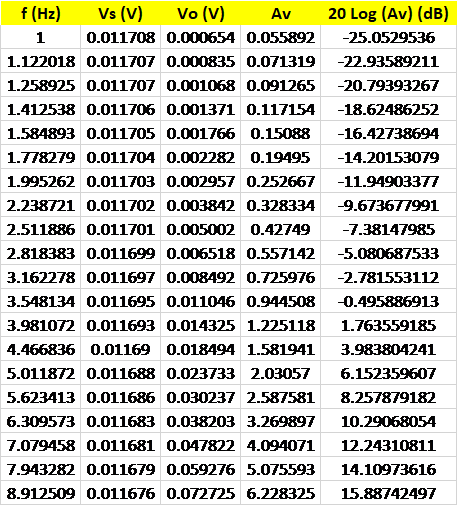
\includegraphics[width=0.4\textheight]{data_cascode_gain.png}
		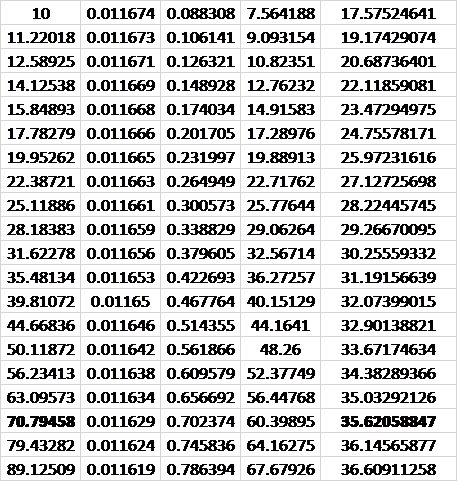
\includegraphics[width=0.4\textheight]{data_cascode_gain_1.png}
		\label{t:4}
	\end{table}

	\pagebreak
	\begin{table}[!ht]
		\centering
		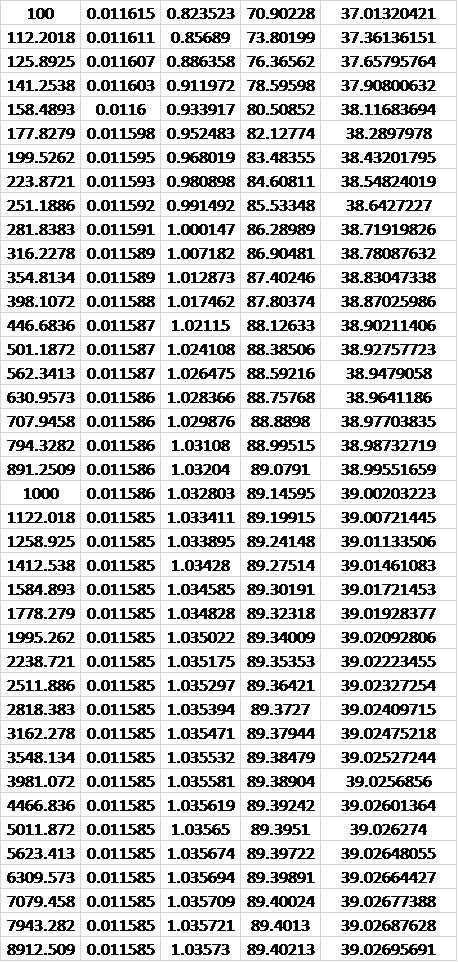
\includegraphics[width=0.4\textheight]{data_cascode_gain_2.png}
	\end{table}
	
	\pagebreak
	\begin{table}[!ht]
		\centering
		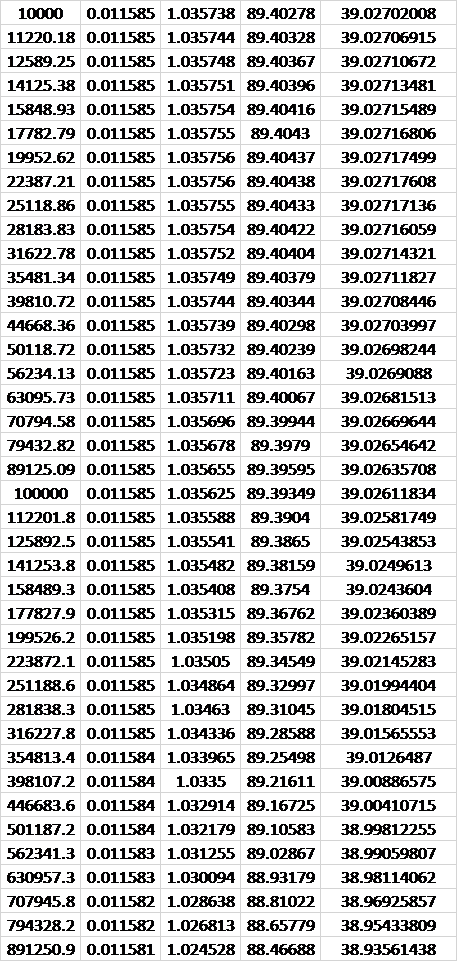
\includegraphics[width=0.4\textheight]{data_cascode_gain_3.png}
	\end{table}

	\pagebreak
	\begin{table}[!ht]
		\centering
		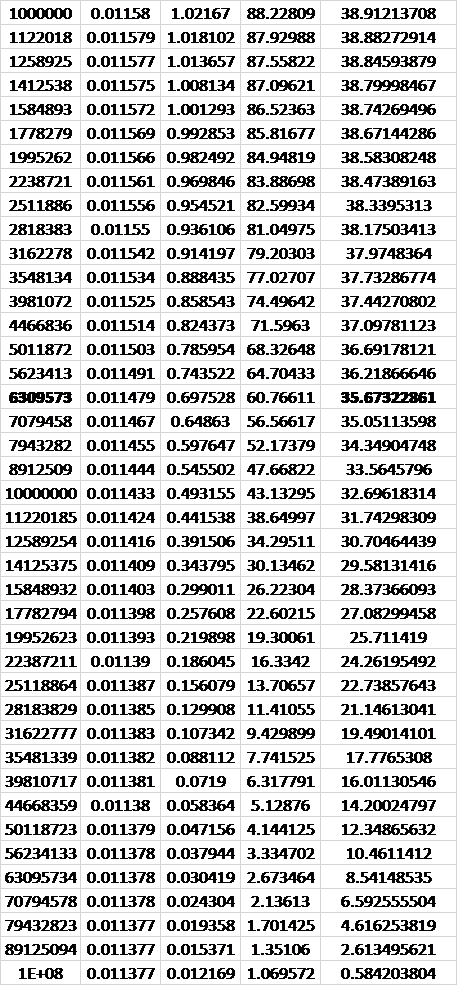
\includegraphics[width=0.4\textheight]{data_cascode_gain_4.png}
	\end{table}

	\pagebreak
	\noindent Using the data presented in Table \ref{t:4}, a plot of the voltage gain vs. frequency was generated as shown below in Figure \ref{f:2}.
	\begin{figure}[!ht]
		\centering
		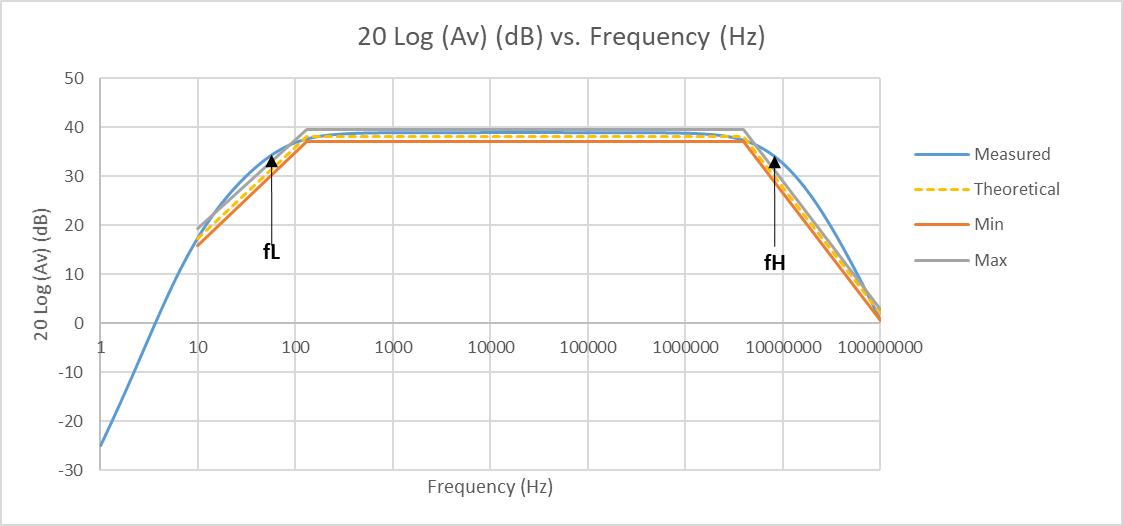
\includegraphics[width=0.7\textheight]{gain_vs_freq.png}
		\captionof{figure}{Voltage Gain vs. Frequency}
		\label{f:2}
	\end{figure}
	
	Table \ref{t:5} below shows the measured data of the gain as a function of the input peak-to-peak voltage swing.
	\begin{table}[!ht]
		\centering
		\captionof{table}{Measured Data of the Gain as a function of input peak-peak Voltage Swing}
		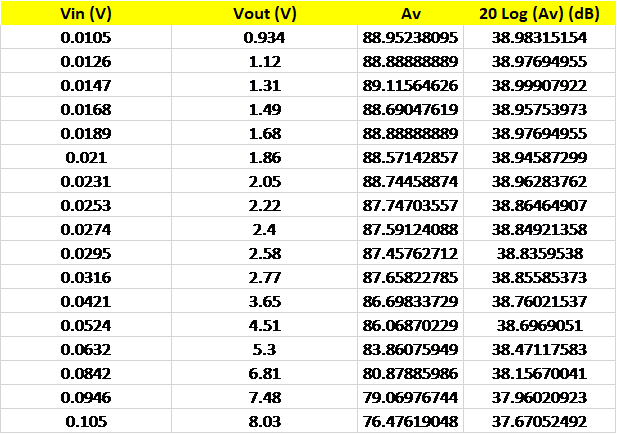
\includegraphics[width=0.8\linewidth]{data_gain_vs_in.png}
		\label{t:5}
	\end{table}
	
	\pagebreak
	\noindent Using the data presented in Table \ref{t:5}, a plot of the voltage gain vs. peak-to-peak voltage swing at the input was generated as shown below in Figure \ref{f:3}.
	\begin{figure}[!ht]
		\centering
		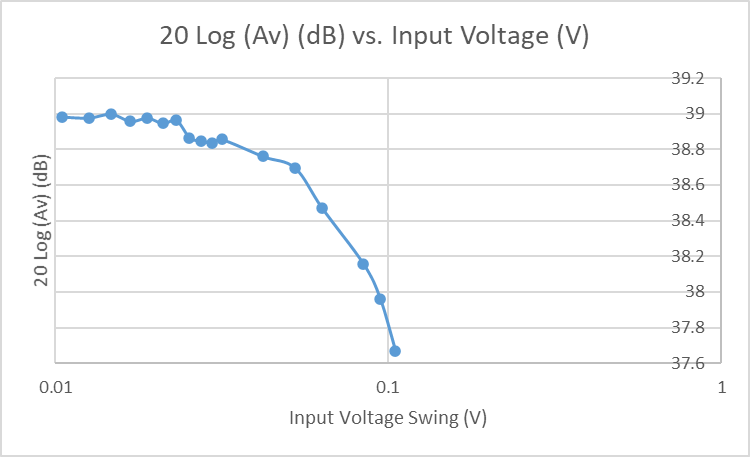
\includegraphics[width=0.6\textheight]{gain_vs_inputVoltageSwing.png}
		\captionof{figure}{Voltage Gain vs. Input Voltage}
		\label{f:3}
	\end{figure}

	\pagebreak
	\subsection*{Discussion}
	\textbf{Amplifier Parameters}\\\\
	As shown in table \ref{t:2}, the achieved gain by the amplifier is 88.12 $v/v$.
	The theoretical gain of the amplifier is (80.05 $\pm$ 10\%) $v/v$.
	This gain falls just into the range required for the gain as the maximum value required for the gain is 88.55 $v/v$.
	Although the measured gain of the amplifier falls within the acceptable range, it does not match the theoretical value exactly due to the assumptions that were made in order to compute the prelab calculations.\\\\
	The measured input impedance is 4.625 k$\Omega$ while the theoretical input impedance is 4.188 k$\Omega$.
	The cause of the difference between the theoretical and measured input impedance can be attributed to the value of $R_S$ as the resistance value was calculated using the theoretical gain of 80.05 $v/v$.\\\\
	The measured output impedance is 4.98 k$\Omega$ which is an exact match of the theoretical output impedance of 5 k$\Omega$.\\\\
	The measured low cutoff frequency is 71 Hz which meets the required specifications as it is below 200 Hz.
	An assumption of the low cutoff frequency of 100 Hz was made in order to compute the prelab calculations which turned out to be a very good assumption as the assumed value is fairly close to the measured one.\\\\
	The measured high cutoff frequency is 6.2 MHz which also meets the required specifications as it is way above 1 MHz.
	However, the theoretical value of the high cutoff frequency is 1.90 MHz.
	The cause of the difference between the theoretical and measured high cutoff frequency can be attributed to the computation of the resistance values of the circuit that the capacitors see.
	It is possible that an error has been made while computing the resutls of the high cutoff frequency.
	However, the measured value of the high cutoff frequency still meets the required specifications of the amplifier design project\\\\
	Another requirement of this amplifier is that the power dissipation of the circuit should not exceed 50 mW.
	The power dissipation calculations for the amplifier circuit can be done as follows:
	\begin{align*}
		P_{DC} &= V_{CC} * I_{CC}\\
		&= V_{CC} * (I_{C} + I_{BB})\\
		&= 15 \hspace{1mm} V * (1 \hspace{1mm} mA + 136 \hspace{1mm}\mu A)\\
		\therefore P_{DC} &= 17.04 \hspace{1mm} mW
	\end{align*}
	\begin{align*}
		P_{ac} &= \frac{v_{o_{rms}}^{2}}{R_{L}}\\
		&= \frac{\left(\frac{2 \hspace{1mm} V_{pk-pk}}{2\sqrt{2}}\right)^{2}}{R_L}\\
		&= \frac{\left(\frac{2 * 2 V}{2\sqrt{2}}\right)^{2}}{15 \hspace{1mm} k\Omega}\\
		\therefore P_{ac} &= 0.13 mW
	\end{align*}
	\begin{align*}
		P &= P_{DC} + P_{ac}\\
		&= 17.04 \hspace{1mm} mW + 0.13 \hspace{1mm} mW\\
		\therefore P &= 17.17 \hspace{1mm} mW
	\end{align*}
	\begin{align*}
		\therefore\eta &= \frac{P_{ac}}{P_{DC}}
		= \frac{0.133}{17.07}
		\approx 0.78\% 
	\end{align*}
	The computed total power dissipation, DC and AC, of the circuit is 17.17 mW which meets the required specifications as it is below 50 mW.
	
	\pagebreak
	
	\noindent\textbf{Voltage Gain vs. Frequency Plot}\\\\
	\noindent Figure \ref{f:2} above shows a plot of the measured gain of the amplifier at various frequencies as well as the theoretical, minimum, and maximum gain that the amplifier is able to achieve based on the given specifications.
	Due to the fact that the measured gain value is very close to the maximum gain value, most of the data points lie along the maximum value line.
	However, most of the data points of the measured gain lie within the range between the minimum and maximum gain value indicating that the amplifier meets the required specifications.\\\\
	
	\noindent\textbf{Voltage Gain vs. Input Voltage Swing Plot}\\\\
	As shown in Figure \ref{f:3} above, at low voltage input, the voltage gain remains fairly constant at around 38.9 dB.
	The point at which the gain differs from the low signal gain by 1 dB at an input voltage of 94.6 mV where the voltage gain is 37.9 dB as shown in Table \ref{t:5} above.
	
	\pagebreak
	
	\section{Conclusion}
	The experiments done in this lab demonstrate the features and characteristics of three basic configurations (CE, CC, and CB) of a signle transistor amplifier.
	They hightlighted the various strengths and weaknesses of each configuration.
	Then, by proper combinations and permutations, 2-transistor amplifier configurations were constructed and studied for improved gain-bandwidth performance [1].
	Finally, a specific configuration of a cascode amplifer was designed to meet or exceed a prescribed set of specifications [1] which presented a great experience with designing, building, and testing an analog circuit.
	
	\pagebreak
	
	\section{References}
	[1] “Lab 2: Amplifier Project” Carleton Univeristy, Ottawa, 2017.	
\end{document}